\documentclass{article}[]
\usepackage[textwidth=15cm]{geometry}
\usepackage[table,xcdraw]{xcolor}
\usepackage{graphicx}
\usepackage{listings}
\usepackage[hidelinks]{hyperref}
\usepackage{pdfpages}
\usepackage{csvsimple}
\usepackage{float}
\usepackage{csquotes}
\makeatletter
\newcommand\urlfootnote@[1]{\footnote{\url@{#1}}}
\DeclareRobustCommand{\urlfootnote}{\hyper@normalise\urlfootnote@}
\makeatother

\begin{document}
	\title{Neural Networks Assignment 3 - Google Deep Dream}
	\author{Anonymous}
	\maketitle
	\lstset{
		basicstyle=\ttfamily,
		keywordstyle=\bfseries,
		language=Java,
		frame=single,
		aboveskip=11pt,
		belowskip=11pt,
		breaklines=true,
		breakatwhitespace=false,
		showspaces=false,
		showstringspaces=false,
		numbers=left,
		stepnumber=1,    
		firstnumber=1,
		numberfirstline=true
	}
	
\section{Abstract}

\section{Introduction}
% neural networks paper für kurs
This paper is the result of fulfilling assignment 3 of the neural networks course at the Universiteit Leiden.
The assignment demands to portray a research topic within the field of neural networks.
We chose to experiment with the visualization of the learned \enquote{knowledge} of a network though \emph{Deep Dream}.

Section \ref{sec:problem-statement} will explain the problems with the lack of knowledge about the encoded data of the trained weights of a neural network.
In section \ref{sec:previous-work} we will look at related work and possible applications.
After that we go deep into the inner workings of the algorithm Deep Dream itself in section \ref{sec:how} to explain how the dreaming works.
We will use and present hand picked images and models, detailed in section \ref{sec:data} to conduct our experiments with. 
The results of these experiments will be displayed in section \ref{sec:evaluation}, and possible conclusions drawn in section \ref{sec:conclusion}.


\subsection{Problem Statement \& Motivation}
\label{sec:problem-statement}
% Warum machen wir das überhaupt?
Neural Networks with meaningful applications are complex structures with many layers, nodes and trained weights.
For example VGG19, an Image Categorisation Neural Network, consists of 19 Layers summing up to a total of 143,667,240 trained parameters\cite{vgg}. These weights were trained to recognize images and map them to a description string based on the ImageNet Dataset.
The problem one faces now is that there is no saying in what the individual layers and nodes have actually learned to respond to, or how the Neural Network actually draws a conclusion\cite{castelvecchi2016can}.
%  -> NN sind Blackboxes, haben zwar definierte Struktur, aber Zusammenspiel der Weights unbekannt
Such behaviour is often referred to as a \textit{black box} and one of the fundamental architectural problems in mastering neural networks\cite{olden2002illuminating}.

% besser nachvollziehen von klassifizierung durch besseres verständnis / visualisierung der gelernten merkmale
In order to get at least a small grasp of what these layers or nodes have learnt, an approach to visualize said knowledge is needed.
As maybe already apparent from the mention of VGG19, we are focusing on neural networks that process images.
Hence the visualization methods that will be portrayed in the coming chapters are limited to image processing neural networks and not generally applicable to \textit{decipher} any neural networks weights.

\subsubsection{Visualizing Learned Features}
% https://blog.keras.io/how-convolutional-neural-networks-see-the-world.html
In this chapter we will describe the visual aspect of the so called \textit{Deep Dream} visualization method.
A detailed mathematical explanation of how and why this works is given in Section \ref{sec:how}.
Deep Dreaming requires a pretrained image recognition neural network, and a source image one wishes to modify. The source image can be any arbitrary image.
Figure \ref{fig:neuronreact} portrays a small section of an abstract unspecified neural network.
The small image parts contained within each neurons are examples of features a neuron can learn to respond to. In this instance the feature was then applied to a random noise image.
One can pick out individual or a set of neurons,
and activate them on the source image to modify it in a way that the learnt features are embedded into it.
An example of this can be seen in Figure \ref{fig:applieddream}.
Here the neuron on the very top left of Figure \ref{fig:neuronreact} was chosen to be activated the most in order to modify the source image and the learnt feature now dominates the visual appearance of the image.
Since it would be close to impossible to find the right combination of neurons to draw a specific object, there is the possibility of a \textit{Guided Dream}.
The concrete inner workings of the \textit{Guided Dream} are explained in Section \ref{guided-dreaming}.
For a guided dream there is a second image in play, which we will refer to as \textit{Guide Image}.
This image is processed by the network and the neurons that responded the most to the features contained within it will then be used for the modification.
That way one could use a blank source image and a guide image, e.g. of a cat. By then selecting the strongest activated neurons by the guide we get an idea of which features the neural network learnt about cats.
An example of this can be seen in Figure \ref{fig:guided}.

\begin{figure}[H]
	\centering
	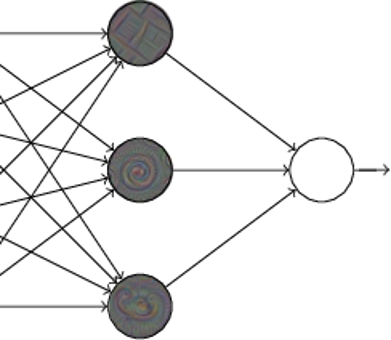
\includegraphics[width=0.5\linewidth]{img/neurons-reaction.png}
	\caption{A small section of an abstract unspecified neural network. Within the layers is the applied \textit{Deep Dream} visualizing the feature learnt by the neuron\cite{nielsen2015neural}.}
	\label{fig:neuronreact}
\end{figure}

\begin{figure}[H]
	\centering
	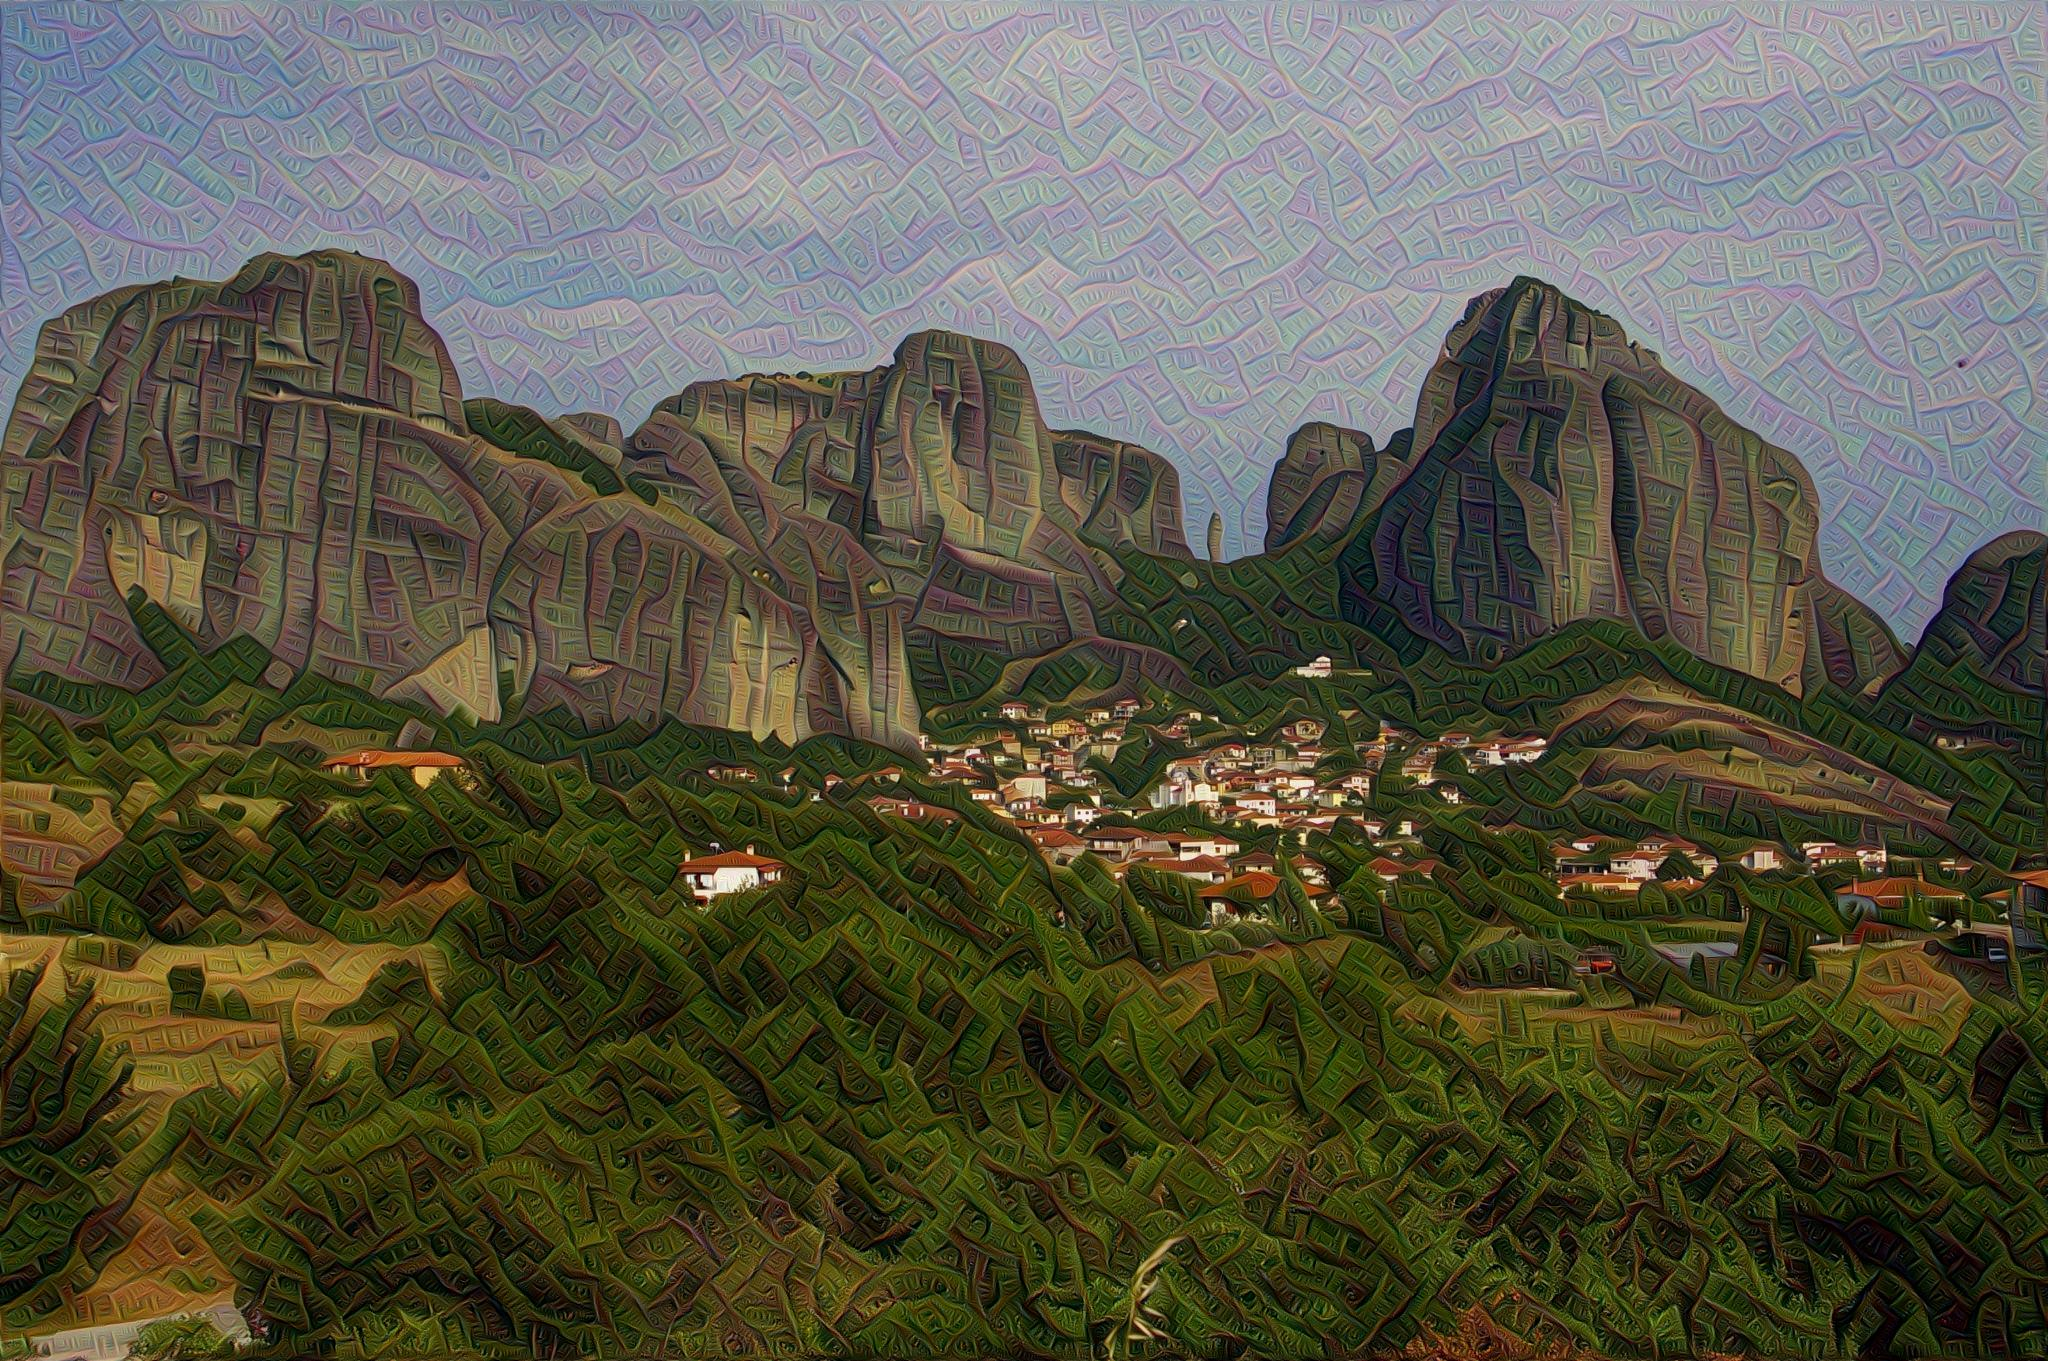
\includegraphics[width=0.5\linewidth]{img/applied_neuron.png}
	\caption{A \textit{Deep Dream} onto a Landscape image as source which maximizes one specific neuron reacting apparently to certain edge types.}
	\label{fig:applieddream}
\end{figure}

% https://research.googleblog.com/2015/06/inceptionism-going-deeper-into-neural.html

% weitere anwendungsbereiche
% interesting results
% fake features for misclassification

\section{Related \& Previous Work}
\label{sec:previous-work}
\subsection{Previous Work}
There are different methods to visualize the content of convolutional neural network.
As explained in Section \ref{sec:how}, \textit{Deep Dream} uses a gradient ascent to achieve its results.
Before the gradient ascent, Zeiler had already developed a method in 2011 called deconvolutional neural networks, to visualize said features\cite{zeiler2011adaptive}.
Simonyan has found that both approaches produce very similar results\cite{simonyan2013deep}.
The reason for that is if that the gradient ascent is a generalisation of the deconvolutional approach.
This generalisation also means that gradient ascent can be applied to any arbitrary layer while the deconvolution is limited to deciphering convolutional layers\cite{simonyan2013deep}.

\subsection{Related Work / Possible Applications}
The visualization of learnt features can be used to achieve different artistic things.
Berov successfully applied \textit{Deep Dreaming} to imitate the visual effects a person might encounter during a hallucination onto any arbitrary image\cite{berov2016visual}.
We subjectively consider some of our results, visible in Section\ref{sec:evaluation}, to also look quite \enquote{trippy} at points which is close to a hallucination.
DiPaola applied \textit{Deep Dreaming} to transform images so they look like they have been painted by a famous painter\cite{dipaola2016using}.
This process is called style transfer and in his experiments DiPaola successfully transformed portrait pictures to look like they were painted by Rembrandt or Freud.




% https://arxiv.org/pdf/1312.6034v2.pdf - Deep Inside Convolutional Networks: Visualising Image Classification Models and Saliency Maps

\section{How Does Dreaming Work}
\label{sec:how}

This section will focus on the main techniques how dreaming actual work.
Similar to the training process of a network, the dreaming algorithm is an optimization problem.
% TODO Formulierung
But rather than training something to classify samples better, the input gets modified in order to get classified more strongly.


\subsection{General}
When looking at the training process of a (Convolutional) Neural Network, one can see that the weights and biases, following only called weights, are changed in such a way that a given error function gets minimized.
Because the error function, for instance \emph{mean squared error}, is rather complex the derivation is very complex if not even infeasible.

% Gradient: Technik um größten Anstieg zu finden -> man nimmt also beim Trainieren den negativen Gradient: -Delta(->W) = [0.2 -1 ...] // GIbt an wie die Weights verändert werden sollten
% Numerische Approximation des Gradients: https://en.wikipedia.org/wiki/Numerical_differentiation
% Gradient Descent/ Full Backpropagation): mache es für alle Trainingsamples und nehme den durchschnitt
% Stochasitic Gradient Descent: Nehm ein paar und nehme den Durchschnitt
% Backpropagation: Determine how one trainign example want to change the weights and biases


That's why the \emph{Gradient descent} algorithm is used to find the (global) minima\footnote{however, using the gradient descent often leads only to a local minima} of the function by taking small steps into the direction of the minima.
This is done by calculating the partial derivatives of the cost function in regard to every weight and bias.

% TODO: mathematische Formeln hinzufügen
In order to do this the learning step can be divided into two essential steps.
First there the \emph{forward} pass, where a sample gets classified by the net.
After that the error made by the network is calculated.
The second step, the \emph{backward} pass, consists of the algorithm of \emph{backpropagation}.
Based on result of the error function, the negative gradient for every weight and bias is calculated.
This can be interpret as the direction in which the function should step in order to decrease that error.
These gradients are added to the weights and bias, which is basically the learning process.
To prevent too slow learning or \enquote{overshooting} local minima a \emph{learning rate} is introduced which gets multiplied with the gradients.

As already said in the introduction of this section, the goal of the Deep Dream technique is not to minimize the cost function, but to modify the input.
Concrete speaking, you choose a layer within the net which output you want to maximize.
We let then the network choose which feature(s) are most present with a given input image at that layer.

% TODO: then use the technique of the backpropagation 

Intuitively this means that we want to increase the features that the network detects such that they are getting more present.
Same as the normal training process of the network, the dreaming is done by using multiple iteration.
%TODO Ref sobald sie da ist
There are also other techniques to improve the results which will be discussed in Section \ref{TODO}


% Add Gradient Descent Image

% TODO: erklären das jitter / image shift dafür da ist, dass übe rmehrere iterationen die änderungen smooth zusammen gehen siehe calc_grad_tiled in https://github.com/tensorflow/tensorflow/blob/master/tensorflow/examples/tutorials/deepdream/deepdream.ipynb


% TODO: Das ist eher eine Konklusion und sollte später bei der Auswertung erwähnt werden
% Einzelne Neuronen identifizieren und deren Features visualisieren, durch Verändern des Input Images, so dass die Neuronen mehr aktiviert werden
% Niedrige Layer enthalten eher abstrakte Features we Linien, Kurven und Ecken während höhere Layer konkrete Features wie z.B. Augen oder Säulen abbilden



% https://github.com/tensorflow/tensorflow/blob/master/tensorflow/examples/tutorials/deepdream/deepdream.ipynb
% Achtung Zitat: 
%\enquote{It consists of a set of layers that apply a sequence of transformations to the input image. The parameters of these transformations were determined during the training process by a variant of gradient descent algorithm. 
% The internal image representations may seem obscure, but it is possible to visualize and interpret them.}


\subsection{Guided Dreaming}
% mit Reference Image
Instead of increasing the occurrence of present features within an image we can also use a reference image in order to achieve \emph{Guided Dreaming}.
For instance if you use a reference picture with animals, the Deep Dreaming algorithm will add animal features the input image that gets modified.


\section{Used Models and Images}
\label{sec:data}
% vortrainierte Neural Networks erklären/erwähnen
% alle basieren auf der Image Database "ImageNet"
For the upcoming experiments in section \ref{sec:evaluation} we need to decide which network model we use and which images are feasible as source or \emph{guide image}.
As classification network we chose to use \emph{ResNet}\cite{he2016deep}, shorthand for \emph{Residual Network}, because it is the current state of the art providing the lowest error rate and hence performs best.\cite{cnnComparison}
It offers three variations differing in the layer amount, namely 50, 101, 152.
Due to performance reasons, see section \ref{sec:performance}, we decided to use the ResNet50.
To apply the \emph{dream} we use a modified version of the original \textit{Google Deep Dream} code\cite{deep-dream-github} for the neural network framework \textit{Caffe}\cite{jia2014caffe}.

By analyzing various existing \emph{dreamed images}, we came to the conclusion that images with a lot of varying objects offering different features might lead to more interesting results.
Hence we were looking for images containing: 
\begin{itemize}
	\item landscape with varying vegetation
	\item houses
	\item water because it offers a lot of noise to act upon
	\item clouds because of the real-life relatability mentioned in section \ref{sec:visual-aspects}
\end{itemize}

To find images with these properties we used \emph{Flickr} because it allows to search for images that are licensed under the \emph{creative commons}.
Figure \ref{fig:imgbeestemarkt} is an image of the Beestenmarkt in Leiden and offers three of the wanted features: water, clouds and buildings.
In addition to that a few people are also present in the picture who might be transformed as well.
The second image, visible in figure \ref{fig:imglandscape}, is a closeup of some vegetation on a field offering a lot of small distinctive features.
It contains two of the features we are looking for, namely a landscape with varying vegetation and houses.
It is also advantageous that the grass is made up of different colors.



\begin{figure}[H]
	\minipage{0.49\textwidth}
	\centering
	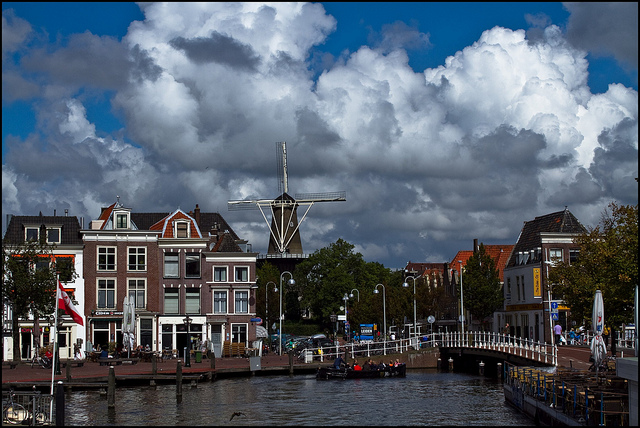
\includegraphics[width=1\linewidth]{img/beestemarkt.jpg}
	\caption{First source image displaying the Beestemarkt in Leiden.\cite{imgbeestemarkt}}
	\label{fig:imgbeestemarkt}
	\endminipage\hfill
	\minipage{0.49\textwidth}
	\centering
	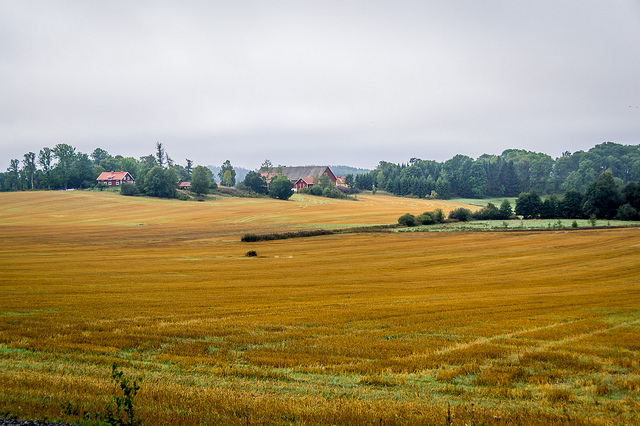
\includegraphics[width=1\linewidth]{img/landscape.jpg}
	\caption{Second source image portraying a landscape with small houses and trees.\cite{imglandscape}}
	\label{fig:imglandscape}
	\endminipage\hfill
\end{figure}

\section{Experiments And Results}
\label{sec:evaluation}
As described in section \ref{sec:visual-aspects} \emph{deep dreaming} works by selecting layers and neurons that should be activated more.
In order to select good layers for the dreaming, we let each layer be dreamt onto an image to handpick the layers that offer interesting features.
Impressive results of that can be seen in section \ref{sec:withoutguide}.

To get a more granular control of the intensified features, one can use a \textit{guide image}.
A \textit{guided dream}, described in section \ref{guided-dreaming}, will select neurons based on the \textit{guide image} in that layer.
The results are presented in section \ref{sec:withguide}.

All images are created using the default parameters given by the \textit{Google Deep Dream} code.
These are 4 \textit{octaves} with a scale factor of 1.4, 10 iterations, a step size of 1.5 and a jitter of 32 pixel.
Experiments with different parameters can be found in section \ref{sec:varying-parameters}.


\subsection{Performance Considerations}
\label{sec:performance}
The runtime of the \textit{Deep Dream} depends mostly on the size of the input image and the layer amount.
Using an image of $\approx$600x430 pixels, 30 layers, 10 iterations and 4 \textit{octaves} can already take around 45 minutes to apply and uses up to 14GB of RAM\footnote{single threaded i7-5930k@3,5GHz, 32GB RAM}.
We also implemented the \textit{bilateral} filter which will be applied after every step.\cite{bilateral}
This will also heavily slow down the runtime because the application of the filter takes a few seconds and is applied at every step of modification.


\subsection{Without Guide Image}
\label{sec:withoutguide}

As mentioned in section \ref{sec:data}, the analyzed model contains 50 layers, so we will not be showing the dreaming results for each one, but rather a selection that we deemed satisfactory.
Throughout these layers one can find all kinds of features varying from different colors, textures to small parts of objects.
Looking at figure \ref{fig:14-landscape} one can see that the recognizable features within a layer are not limited to a particular one and includes transitions between the different textures.
These transitions seem to distinguish pixelated regions from very sharp ones.
But it can also result in a transition from smooth curves to very straight lines \ref{fig:16-landscape}.

\begin{figure}[H]
	\minipage{0.32\textwidth}
	\centering
	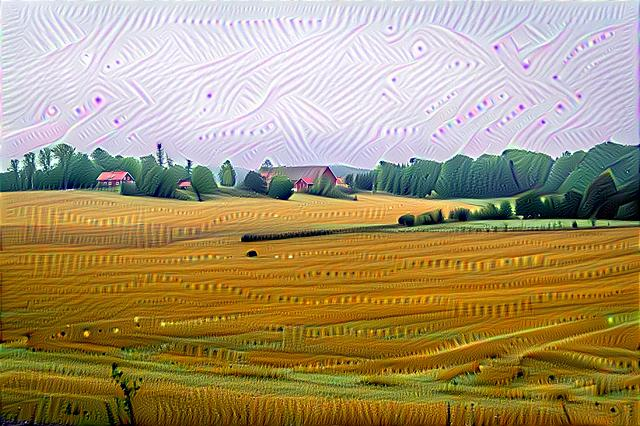
\includegraphics[width=1\linewidth]{img/alpsted-landscape_res3a_branch1.jpg}
	\caption{Dreamed onto the field with layer 12 \enquote{res3a\_branch1}.}
	\label{fig:layer-artistic}
	\endminipage\hfill
	\minipage{0.32\textwidth}
	\centering
	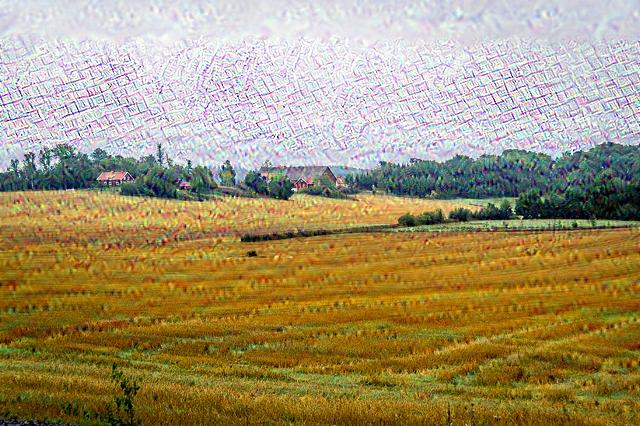
\includegraphics[width=1\linewidth]{img/14_alpsted-landscape_res3a_branch2b.jpg}
	\caption{Dreamed onto the field with layer 14 \enquote{res3a\_branch2b}.}
	\label{fig:14-landscape}
	\endminipage\hfill
	\minipage{0.32\textwidth}
	\centering
	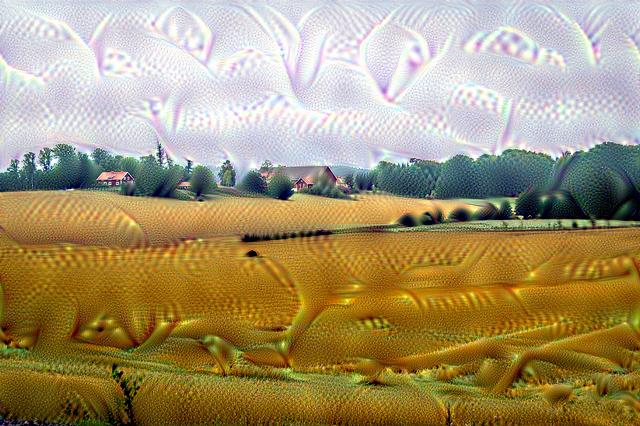
\includegraphics[width=1\linewidth]{img/16_alpsted-landscape_res3b_branch2a.jpg}
	\caption{Dreamed onto the field with layer 16 \enquote{res3b\_branch2a}.}
	\label{fig:16-landscape}
	\endminipage\hfill
\end{figure}


Going further up in the layers we found one layer of particular interest, depicted in figure \ref{fig:layer-snake}.
It visualizes four distinct things at once which makes it unique.
There is a snake's head in the lower left part of the image as well as to the right of the very left house.
The field and large parts of the sky were transformed to look like snake scales.
Apart from these two already distinctive objects the center seems to contain the right part of a dog's face and above it, the sky looks more like dog fur.

Another interesting find is layer 12 depicted in figure \ref{fig:layer-artistic}.
If one ignores the lines and purple tint it looks like an artistic style filter was applied.
This supports DiPaolo's findings, mentioned in section \ref{sec:previous-work}, that by using the right combination of neurons \textit{deep dream} can be used to modify pictures such that they look like paintings.

Another applied change that can be observed in almost all layers is a slight purple to rainbowish tint that gets applied to the image, especially around the newly added features, as visible within the lines in figure \ref{fig:layer-artistic} and in the sky of figure \ref{fig:layer-snake}.

\begin{figure}[H]
	\centering
	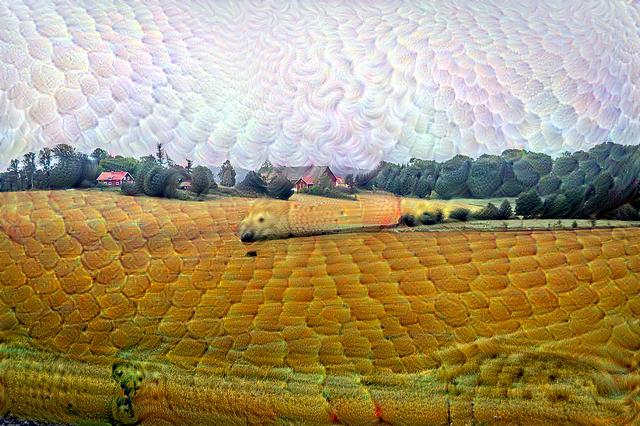
\includegraphics[width=0.7\linewidth]{img/alpsted-landscape_res4f_branch2a.jpg}
	\caption{Layer 41 \emph{res4f\_branch2a}. Seems like snake scales with a snake head in the lower left.}
	\label{fig:layer-snake}
\end{figure}


\subsection{Varying Parameters}
\label{sec:varying-parameters}
In section \ref{sec:optimizations}, we mentioned the varying parameters that can be used to optimize the results, hence we will experiment with them here.

Playing around with the iterations

To show the effect of more iterations, we have increased them by a factor of ten (100 total).
This results in images, where few of the original aspects are still visible, but the learned features dominate the visual appearance.
This can be very well seen in figure \ref{fig:baum}
Here branches of a tree prevail the sky and the field was replaced by shrubs.
The houses have been eradicated by trees.

\begin{figure}[H]
	\centering
	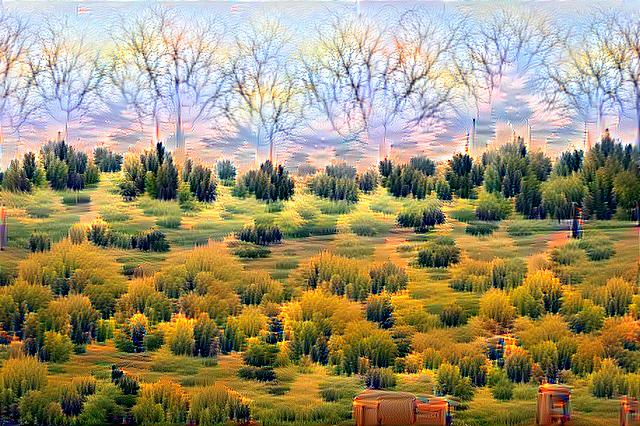
\includegraphics[width=0.7\linewidth]{img/baum}
	\caption{Layer 37 \enquote{res4d\_branch2c}}
	\label{fig:baum}
\end{figure}

Sometimes higher iterations are not sufficient to fully transform every aspect of an image.
This can be seen in figure \ref{fig:houses1} at the houses on the left, that remain almost untouched.
When we also increase the step size from 1.4 to 2.0 we were able to modify the image beyond recognition, see figure \ref{fig:houses2}.
By increasing both parameters, we were able to clearly visualize the learned features within the layer.


\begin{figure}[H]
	\minipage{0.49\textwidth}
	\centering
	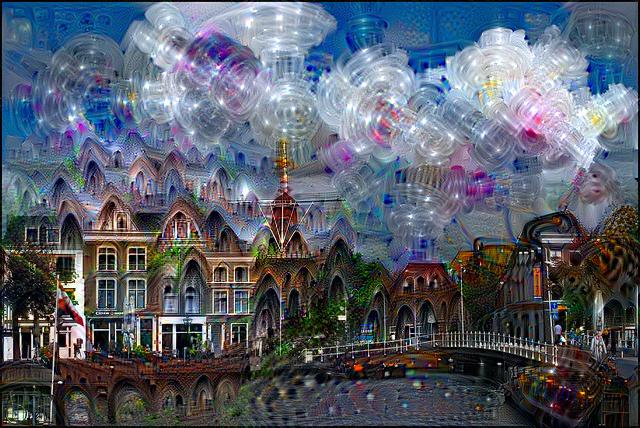
\includegraphics[width=1\linewidth]{img/houses1.jpg}
	\caption{Dreamed onto the Beestenmarkt with layer 43 \enquote{res4f\_branch2c} with step size 1.4.}
	\label{fig:houses1}
	\endminipage\hfill
	\minipage{0.49\textwidth}
	\centering
	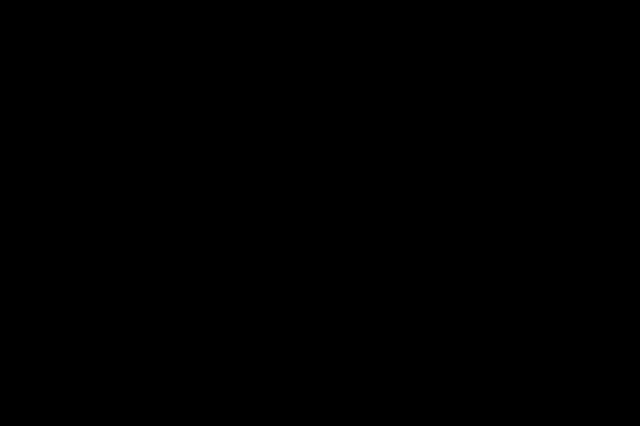
\includegraphics[width=1\linewidth]{img/houses2.jpg}
	\caption{Dreamed onto the Beestenmarkt with layer 43 \enquote{res4f\_branch2c} with \textit{step size} 2.0.}
	\label{fig:houses2}
	\endminipage\hfill
\end{figure}

TODO: bilateral


\subsection{With Guide Image}
\label{sec:withguide}
Following up on section \ref{guided-dreaming}, we want highlight the possibilities opened up through \textit{guided dreaming}.
We decided to choose a picture of puppies, because the ImageNet dataset contains a large amounts of varying dog breeds.
Because we let each layer be dreamt onto an image, we could select one that seems to resemble dogs or animals.
We ended up choosing layer 33 \enquote{res4c\_2b}.
As one can see, by using only 50 iterations in combination with a \textit{guide image}, feature of dogs overshadows the original image.

We also evaluated the effect of increased step size, but omitted the results because the visual difference was not nearly as clear as in the previous section.

\begin{figure}[H]
	\minipage{0.40\textwidth}
	\centering
	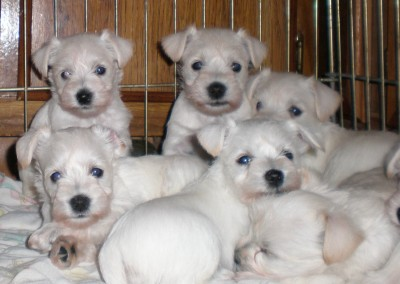
\includegraphics[width=1\linewidth]{img/guide.jpg}
	\caption{Guide image\cite{imgpuppies}}
	\label{fig:guide}
	\endminipage\hfill
	\minipage{0.59\textwidth}
	\centering
	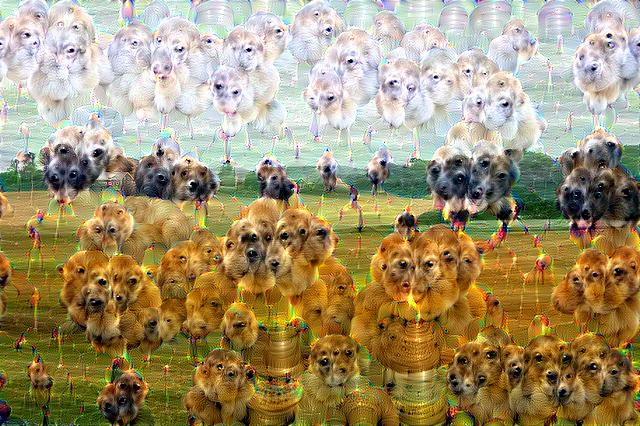
\includegraphics[width=1\linewidth]{img/guide_dream.jpg}
	\caption{Dreamed onto the Field with layer 33 \enquote{res4c\_branch2b} using the \textit{guide image}.}
	\label{fig:guide_dream}
	\endminipage\hfill
\end{figure}



\subsection{Repeating Features}
\label{sec:repeating-features}

Within the different layers we found some to behave quite similar.
Previously we presented layers that differ from each other in form, size and shape.
Here we present layers that seem to have learned almost the same features.
To show the behavior in the clearest way possible we applied dreaming onto the same random generated noise.
As one can see in the figures \ref{fig:rotated_feature_1} \ref{fig:rotated_feature_2}, the created images look almost the same, the only real difference is the orientation.
It looks the enhanced features were simply rotated.

\begin{figure}[H]
	\minipage{0.49\textwidth}
	\centering
	
\includegraphics[width=1\linewidth]{img/rotated_feature_1.jpg}
	\caption{Dreamed onto random now with the \enquote{res2c\_branch2b} layer}
	\label{fig:rotated_feature_1}
	\endminipage\hfill
	\minipage{0.49\textwidth}
	\centering
	
\includegraphics[width=1\linewidth]{img/rotated_feature_2.jpg}
	\caption{Dreamed onto random now with the \enquote{res2c\_branch2c} layer}
	\label{fig:rotated_feature_2}
	\endminipage\hfill
\end{figure}



\section{Conclusion}
\label{sec:conclusion}
This section is about the observations and conclusion that were made while working on and with Deep Dream.

% Test: Image modifizieren mit dem Ziel es bestimmt Klassifizieren zu lassen, anschließend diese Behauptung prüfen
Generally speaking one can see that lower layers tend to select more abstract features such as lines, curves, waves or textures, while higher layers often select more concrete features such as eyes, body parts of animals or vegetation\footnote{we refer lower layers with the early ones and higher layers with later ones during a forward pass}.
Examples for this were presented in section \ref{sec:evaluation}.
The presented related work from section \ref{sec:previous-work} generates videos using Deep Dream.
It makes this fact very clear, because it slowly walks from the lower to the higher layers.
This lets one clearly see the different levels of abstraction encoded in the layers.

We have shown that by increasing certain parameters images can be altered so strongly, that the original can barely be recognized anymore (section \ref{sec:withoutguide}).
It was also shown, that the features from a \emph{guide image} can successfully be transferred onto the target using Deep Dream in section \ref{sec:withguide}.

As described in section \ref{sec:repeating-features}, some learned features seem to repeat across layers in a rotated way.
This observation supports a claim that was found in the Keras blog.\cite{keras-blog}
They found that convolutional layers are not rotation invariant and hence features repeat over the layers.
If one were able to find a method to make them rotation invariant, it could reduce the required layer amount by a large factor.




\bibliography{report} 
\bibliographystyle{ieeetr}
	
	
\end{document}